
We consider the Rosenbrock function for $\boldsymbol{x} \in \mathbbm{R}^2$
\begin{equation*}
    f(\boldsymbol{x})=100(x_2-x_1^2)^2+(1-x_1)^2
\end{equation*}
with two different starting point $\boldsymbol{x}^{(0)}=(1.2,1.2)$ and $\boldsymbol{x}^{(0)}=(-1.2,1)$.
\\
The global minima for the function is zero and the global minimum
point is $\boldsymbol{x^*}=(1,1)$, as shown in the following figure.

\begin{figure}[H]
    \centering
    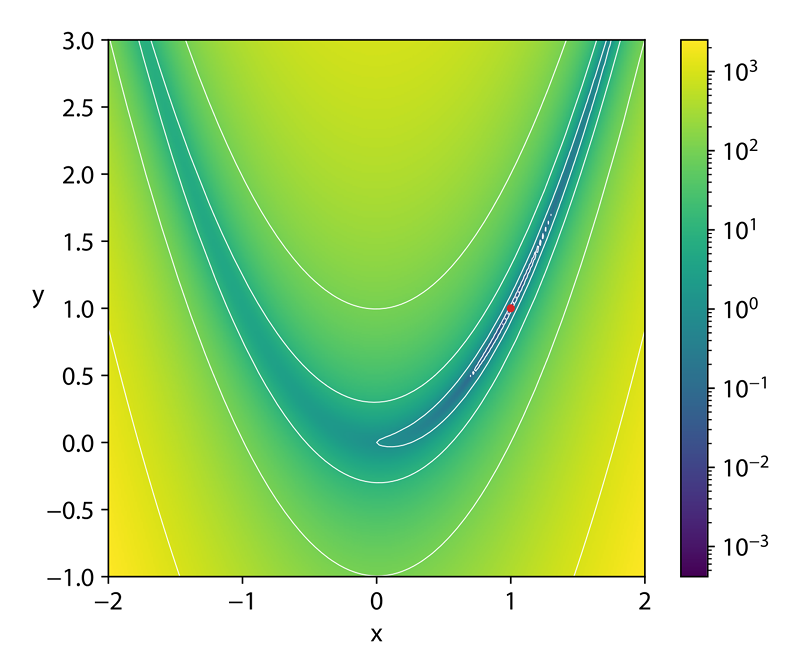
\includegraphics[width=0.4\textwidth]{img/es2_function.png}
    \caption{Rosenbrock function, top view.} 
    \label{pb 2 graph}
\end{figure}

For the Nelder-Mead method we use 400 as maximum number of iterations and the default parameters 
for reflection, expansion, contraction and shrinking; which are respectively
\begin{eqnarray*}
    \rho &=& 1 \\
    \chi &=& 2 \\
    \gamma &=& 0.5 \\
    \sigma &=& 0.5
\end{eqnarray*}
For the Modified Newton method, 5000 maximum outer iterations, 100 maximum iterations allowed to 
compute tra matrix $B_k$ at every step $k$. For backtracking we used the following values of the parameters 
\begin{eqnarray*}
    \rho &=& 0.5 \\
    c_1 &=& 10^{-4} \\
    \texttt{btmax} &=& 40
\end{eqnarray*}
where \texttt{btmax} is the maximum number of iterations allowed for backtracking and is chosen 
in such a way that stagnation is not allowed ($\rho^{\texttt{btmax}}\approx 10^{-13}>\epsilon_m$ 
where $\epsilon_m \approx 10^{-16}$ is the machine precision).
\\
For both methods the tolerance used is $10^{-7}$.

Computing the average for each method on the two runs, we obtain the following results:
\begin{figure}[H]
    \centering
    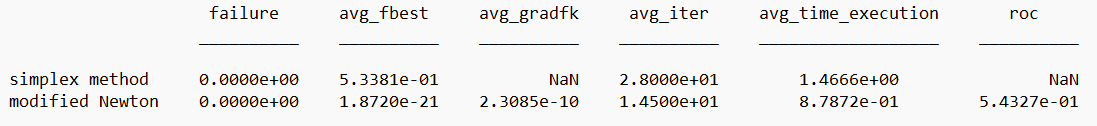
\includegraphics[width=\textwidth]{img/es2_table.png}
    \caption{Results obtained by running both methods on the Rosenbrock function.} 
    \label{pb 2 table}
\end{figure}
Both method were able to find a good approximation of the solution within the maximum number 
of iterations allowed. The Modified Newton method is in this case faster because it exploits 
the information contained in the gradient and the Hessian matrix, without the burden of costly 
operations that would occur in bigger dimension. However the rate of convergence is lower than the
theoretical one. For the Nelder-Mead method it is \texttt{NaN} because this methods allows for 
consecutive iterations to have the same value of the current solution $x^{(k)}$, resulting in a 
division by zero when applying the formula $\eqref{definizione_roc}$.
